\documentclass[tikz,border=2mm]{standalone}
\usepackage{pgfplots}
\begin{document}
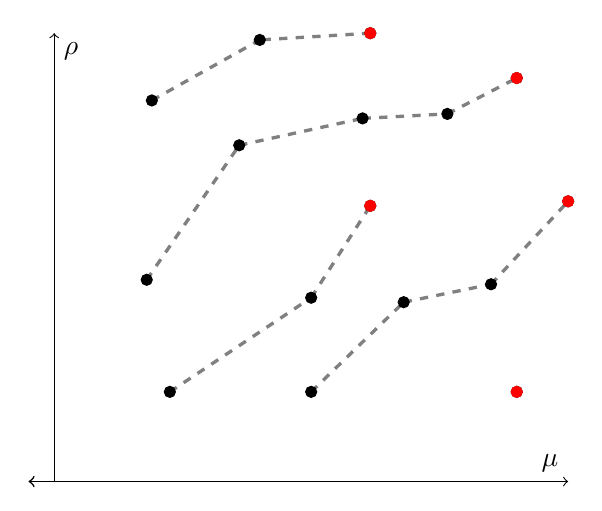
\begin{tikzpicture}

\begin{axis}[
    axis lines = center,
    axis line style = {->},
    xlabel = $\mu$,
    ylabel = {$\rho$},
    xmin=-1, xmax=20,
    ymin=0, ymax=20,
    xtick=\empty, ytick=\empty,
    clip=false
]
\addplot [only marks] table {
    3.8 17
    8 19.7
    12.3 20

    3.6 9
    7.2 15
    12 16.2
    15.3 16.4
    18 18

    4.5 4
    10 8.2
    12.3 12.3

    10 4
    13.6 8
    17 8.8
    20 12.5

    18 4
};
\addplot [only marks, red] table {
     12.3 20
     18 18
     12.3 12.3
     20 12.5
     18 4
};

\draw[->, semithick] (0,0) -- (-1,0);

\draw[dashed, color=gray, very thick] (axis cs:3.8,17) -- (axis cs:8,19.7);
\draw[dashed, color=gray, very thick] (axis cs:12.3,20) -- (axis cs:8,19.7);

\draw[dashed, color=gray, very thick] (axis cs:3.6,9) -- (axis cs:7.2,15);
\draw[dashed, color=gray, very thick] (axis cs:7.2,15) -- (axis cs:12,16.2);
\draw[dashed, color=gray, very thick] (axis cs:12,16.2) -- (axis cs:15.3,16.4);
\draw[dashed, color=gray, very thick] (axis cs:15.3,16.4) -- (axis cs:18,18);

\draw[dashed, color=gray, very thick] (axis cs:4.5,4) -- (axis cs:10,8.2);
\draw[dashed, color=gray, very thick] (axis cs:10,8.2) -- (axis cs:12.3,12.3);

\draw[dashed, color=gray, very thick] (axis cs:10,4) -- (axis cs:13.6,8);
\draw[dashed, color=gray, very thick] (axis cs:13.6,8) -- (axis cs:17,8.8);
\draw[dashed, color=gray, very thick] (axis cs:17,8.8) -- (axis cs:20,12.5);



\end{axis}
\end{tikzpicture}
\end{document}


